\documentclass{article}

% packages
\usepackage{amsmath, amsthm, thmtools, amsfonts, amssymb, luacode, catchfile, tikzducks, hyperref, ifthen}
\ifcsname c@kobocompile\endcsname
	\usepackage[a5paper, total={1072pt, 1448pt}, margin=10pt, includeheadfoot]{geometry} % set page margins
\else
	\usepackage[a4paper, margin=50pt, includeheadfoot]{geometry}
\fi
\usepackage[shortlabels]{enumitem}
\usepackage[skip=3pt, indent=0pt]{parskip}

% language
\usepackage[bidi=basic, layout=tabular, provide=*]{babel}
\ifcsname c@english\endcsname
	\babelprovide[main, import]{english}
\else
	\babelprovide[main, import]{hebrew}
	\babelprovide{rl}
\fi
%\babelfont{rm}{Libertinus Serif}
\babelfont{rm}[Renderer=Harfbuzz]{Libertinus Serif}
\babelfont{sf}{Libertinus Sans}
\babelfont{tt}{Libertinus Mono}

% style
\AddToHook{cmd/section/before}{\clearpage}	% Add line break before section
\linespread{1.3}
\setcounter{secnumdepth}{0}		% Remove default number tags from sections, this won't do well with theorems
\AtBeginDocument{\setlength{\belowdisplayskip}{3pt}}
\AtBeginDocument{\setlength{\abovedisplayskip}{3pt}}
\graphicspath{ {../images/} }

% operators
\DeclareMathOperator\cis{cis}
\DeclareMathOperator\Sp{Sp}
\DeclareMathOperator\tr{tr}
\DeclareMathOperator\im{Im}
\DeclareMathOperator\re{Re}
\DeclareMathOperator\diag{diag}
\DeclareMathOperator*\lowlim{\underline{lim}}
\DeclareMathOperator*\uplim{\overline{lim}}
\DeclareMathOperator\rng{rng}
\DeclareMathOperator\Sym{Sym}
\DeclareMathOperator\Arg{Arg}
\DeclareMathOperator\Log{Log}
\DeclareMathOperator\dom{dom}
\DeclareMathOperator\supp{Supp}
\DeclareMathOperator\var{Var}
\DeclareMathOperator\cov{Cov}

% commands
%\renewcommand\qedsymbol{\textbf{מש''ל}}
%\renewcommand\qedsymbol{\fbox{\emoji{lizard}}}
\newcommand{\Aa}[0]{\mathcal{A}}
\newcommand{\Bb}[0]{\mathcal{B}}
\newcommand{\CC}[0]{\mathbb{C}}
\newcommand{\Cc}[0]{\mathcal{C}}
\newcommand{\EE}[0]{\mathbb{E}}
\newcommand{\FF}[0]{\mathbb{F}}
\newcommand{\Ff}[0]{\mathcal{F}}
\newcommand{\Ii}[0]{\mathcal{I}}
\newcommand{\Gg}[0]{\mathcal{G}}
\newcommand{\Ll}[0]{\mathcal{L}}
\newcommand{\Mm}[0]{\mathcal{M}}
\newcommand{\NN}[0]{\mathbb{N}}
\newcommand{\Nn}[0]{\mathcal{N}}
\newcommand{\PP}[0]{\mathbb{P}}
\newcommand{\Pp}[0]{\mathcal{P}}
\newcommand{\QQ}[0]{\mathbb{Q}}
\newcommand{\RR}[0]{\mathbb{R}}
\newcommand{\Rr}[0]{\mathcal{R}}
\newcommand{\Ss}[0]{\mathcal{S}}
\newcommand{\TT}[0]{\mathbb{T}}
\newcommand{\Uu}[0]{\mathcal{U}}
\newcommand{\Vv}[0]{\mathcal{V}}
\newcommand{\Ww}[0]{\mathcal{W}}
\newcommand{\ZZ}[0]{\mathbb{Z}}
\newcommand{\acts}[0]{\circlearrowright}
\newcommand{\explain}[2] {
	\begin{flalign*}
		 && \text{#2} && \text{#1}
	\end{flalign*}
}
\newcommand{\maketitleprint}[0]{ \begin{center}
	%\begin{tikzpicture}[scale=3]
	%	\duck[graduate=gray!20!black, tassel=red!70!black]
	%\end{tikzpicture}	
	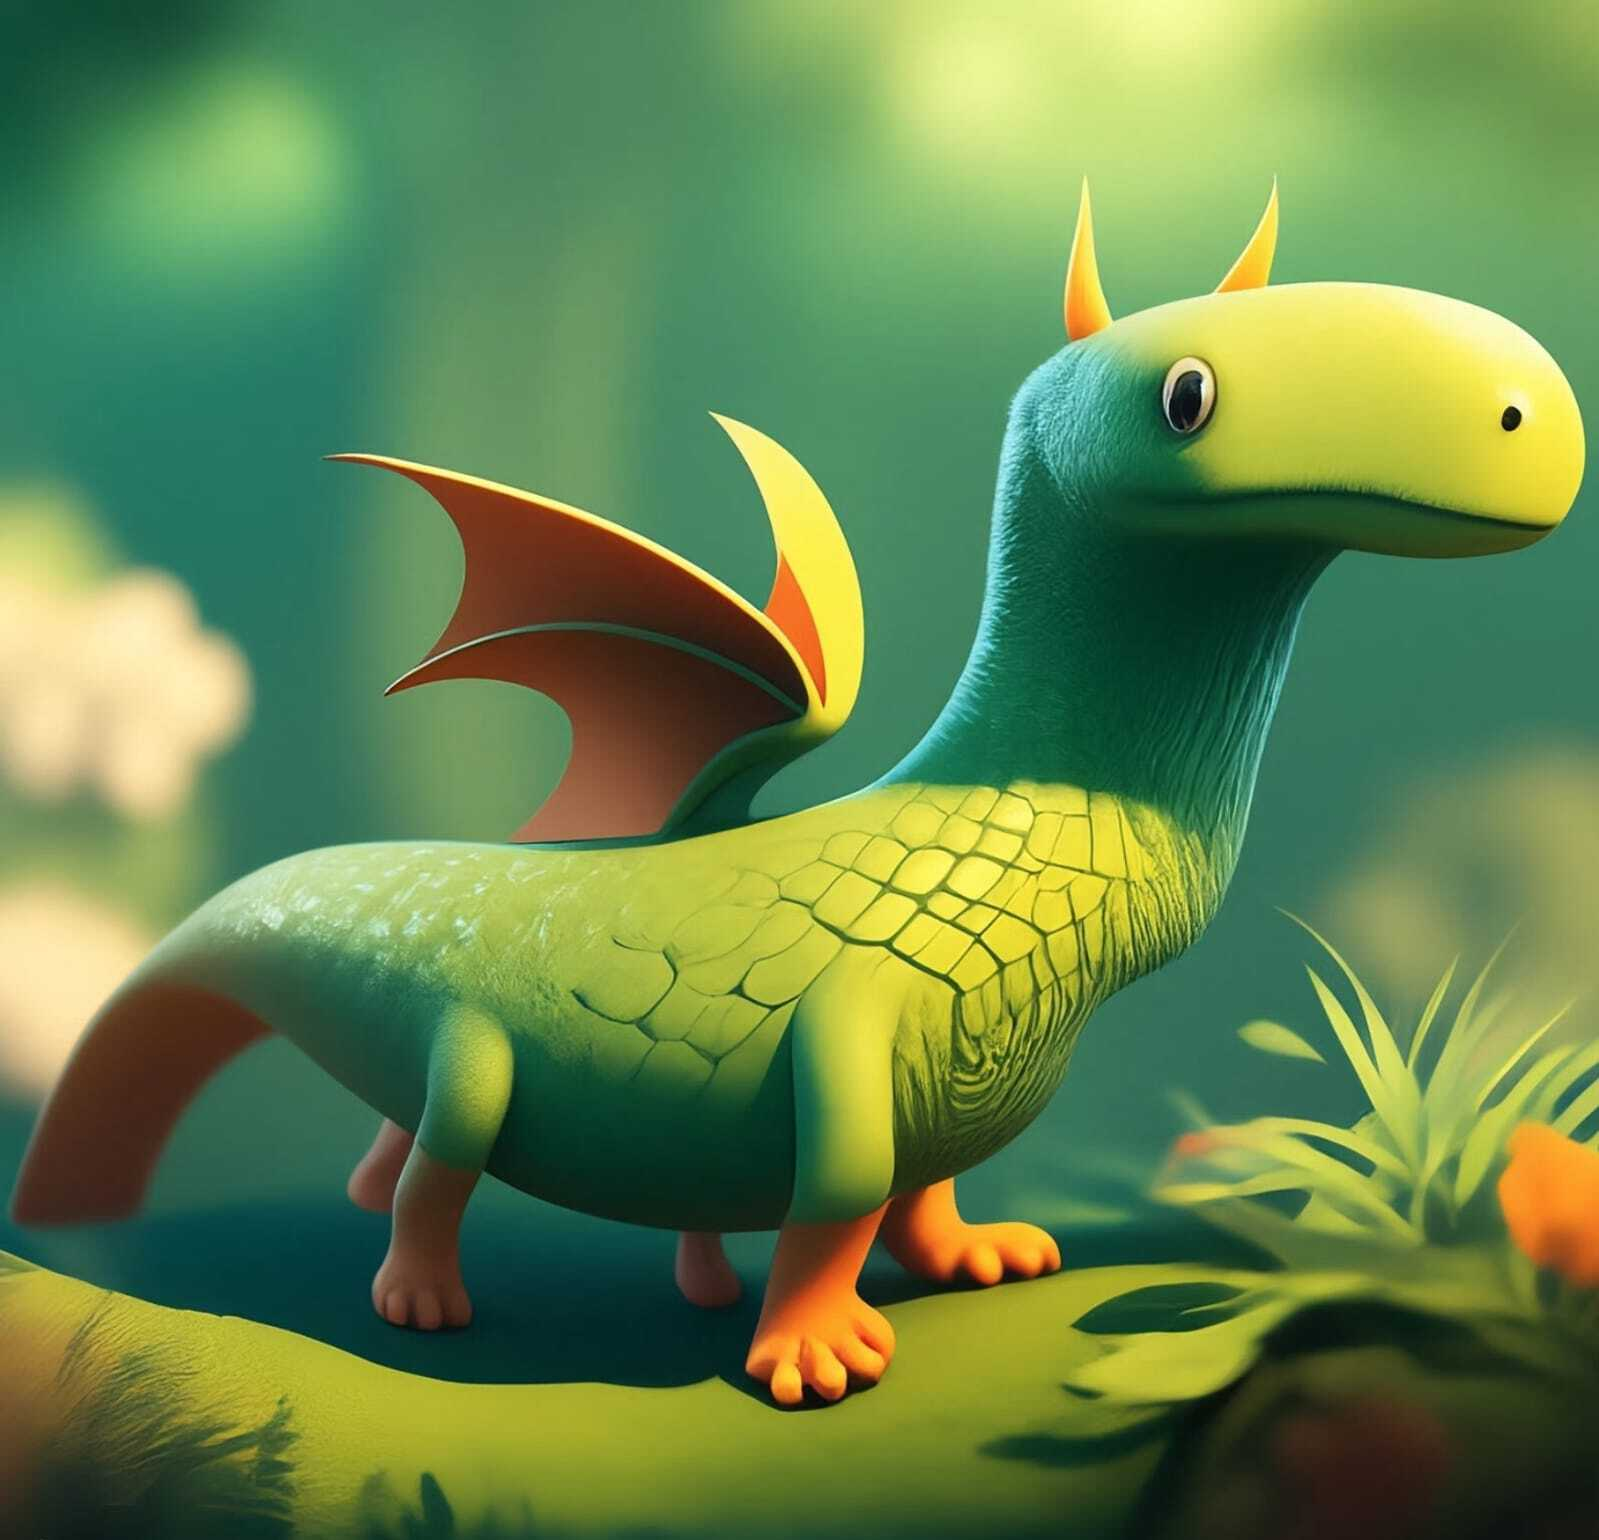
\includegraphics[width=6cm]{cover}
\end{center}
}

% theorem commands
\newtheoremstyle{c_remark}
	{}	% Space above
	{}	% Space below
	{}% Body font
	{}	% Indent amount
	{\bfseries}	% Theorem head font
	{}	% Punctuation after theorem head
	{.5em}	% Space after theorem head
	{\thmname{#1}\thmnumber{ #2}\thmnote{ \normalfont{\text{(#3)}}}}	% head content
\newtheoremstyle{c_definition}
	{3pt}	% Space above
	{3pt}	% Space below
	{}% Body font
	{}	% Indent amount
	{\bfseries}	% Theorem head font
	{}	% Punctuation after theorem head
	{.5em}	% Space after theorem head
	{\thmname{#1}\thmnumber{ #2}\thmnote{ \normalfont{\text{(#3)}}}}	% head content
\newtheoremstyle{c_plain}
	{3pt}	% Space above
	{3pt}	% Space below
	{\itshape}% Body font
	{}	% Indent amount
	{\bfseries}	% Theorem head font
	{}	% Punctuation after theorem head
	{.5em}	% Space after theorem head
	{\thmname{#1}\thmnumber{ #2}\thmnote{ \text{(#3)}}}	% head content

\ifcsname c@english\endcsname
	\theoremstyle{plain}
	\newtheorem{theorem}{Theorem}[section]
	\newtheorem{lemma}[theorem]{Lemma}
	\newtheorem{proposition}[theorem]{Proposition}
	\newtheorem*{proposition*}{Proposition}
	%\newtheorem{corollary}[theorem]{אין חלופה עברית}

	\theoremstyle{definition}
	\newtheorem{definition}[theorem]{Definition}
	\newtheorem*{definition*}{Definition}
	\newtheorem{example}{Example}[section]
	\newtheorem{exercise}{Exercise}[section]

	\theoremstyle{remark}
	\newtheorem*{remark}{Remark}
	\newtheorem*{solution}{Solution}
	\newtheorem{conclusion}[theorem]{Conclusion}
	\newtheorem{notation}[theorem]{Notation}
\else
	\theoremstyle{c_plain}
	\newtheorem{theorem}{משפט}[section]
	\newtheorem{lemma}[theorem]{למה}
	\newtheorem{proposition}[theorem]{טענה}
	\newtheorem*{proposition*}{טענה}
	%\newtheorem{corollary}[theorem]{אין חלופה עברית}

	\theoremstyle{c_definition}
	\newtheorem{definition}[theorem]{הגדרה}
	\newtheorem*{definition*}{הגדרה}
	\newtheorem{example}{דוגמה}[section]
	\newtheorem{exercise}{תרגיל}[section]

	\theoremstyle{c_remark}
	\newtheorem*{remark}{הערה}
	\newtheorem*{solution}{פתרון}
	\newtheorem{conclusion}[theorem]{מסקנה}
	\newtheorem{notation}[theorem]{סימון}
\fi

% Questions related commands
\newcounter{question}
\setcounter{question}{1}
\newcounter{sub_question}
\setcounter{sub_question}{1}

\ifcsname c@english\endcsname
	\newcommand{\question}[1][0]{
		\ifthenelse{#1 = 0}{}{\setcounter{question}{#1}}
		\section{Question \arabic{question}}
		\addtocounter{question}{1}
		\setcounter{sub_question}{1}
	}

	\newcommand{\subquestion}[1][0]{
		\ifthenelse{#1 = 0}{}{\setcounter{sub_question}{#1}}
		\subsection{Part \alph{sub_question}}
		\addtocounter{sub_question}{1}
	}
\else
	\newcommand{\question}[1][0]{
		\ifthenelse{#1 = 0}{}{\setcounter{question}{#1}}
		\section{שאלה \arabic{question}}
		\addtocounter{question}{1}
		\setcounter{sub_question}{1}
	}

	\newcommand{\subquestion}[1][0]{
		\ifthenelse{#1 = 0}{}{\setcounter{sub_question}{#1}}
		\subsection{סעיף \localecounter{letters.gershayim}{sub_question}}
		\addtocounter{sub_question}{1}
	}
\fi

% import lua and start of document
\directlua{common = require ('../common')}

\GetEnv{AUTHOR}

% headers
\author{\AUTHOR}
\date\today

\title{פתרון מטלה 06 --- מבנים אלגבריים 1 (80445)}

\begin{document}
\maketitle
\maketitleprint{}

\Question{}
\Subquestion{}
נוכיח שלכל $n \ge 1$, החבורה $\ZZ_{/n}$ מכילה תת־חבורה יחודית מסדר $d$ לכל $d \mid n$.
\begin{proof}
	יהי $d \mid n$, ונגדיר גם $k = \frac{n}{d}$.
	אנו יודעים כי $\ZZ / n\ZZ \cong \ZZ_{/n}$ ונבחן את $d\ZZ_{/n}$, דהינו $d\ZZ/n\ZZ$, 
	ממשפט האיזומורפיזם השלישי נקבל כי $(\ZZ / n\ZZ) / (d\ZZ / n\ZZ) \cong \ZZ_{/d}$. \\*
	נוכל אם כן להניח ש־$d\ZZ_{/n}$ היא מסדר $d$ אף היא, ואנו יודעים כי היא אכן תת־חבורה של $\ZZ_{/n}$, נותר להראות כי היא יחידה. \\*
	תהי תת־חבורה אחרת $H$ של $\ZZ_{/n}$ אשר היא מסדר $d$, אז קיים איבר $a \in H$ כך שהסדר שלו הוא $d$, זאת אנו יודעים מהתכונות של $\ZZ_{/n}$, ואנו יודעים כי $a \in d\ZZ_{/n}$ ולכן נוכל להסיק כי תת־החבורות שוות.
\end{proof}

\Subquestion{}
נוכיח כי $a \in \ZZ_{/n}$ יוצר תת־חבורה מסדר $d$ אם ורק אם $\gcd(a, n) = \frac{n}{d}$.
\begin{proof}
	\textbf{כיוון ראשון:}
	נניח כי $a$ יוצר תת־חבורה מסדר $d$, ולכן נוכל להסיק מהסעיף הקודם כי $d \mid a \mid n$, ולכן נשתמש במסקנה מהרצאה ונקבל $\gcd(a, d) = 1$, ומכאן נוכל להסיק את המבוקש ישירות.

	\textbf{כיוון שני:}
	נניח כי $\gcd(a, n) = \frac{n}{d}$, לכן נוכל להסיק כי $\frac{n}{d} \in \ZZ_{/n}$, וכי $\frac{n}{d}$ הוא מסדר $d$, ולכן נוכל להסיק כי $a$ עצמו יוצר תת־חבורה מסדר זה.
\end{proof}

\Subquestion{}
נוכיח כי $Aut(\ZZ_{/n}) \cong {(\ZZ_{/n})}^\times$ כאשר זו מוגדרת על־ידי חבורת האלמנטים $1 \le a \le n - 1$ אשר הם ראשוניים זרים ל־$n$ עם כפל מודולו $n$.

\Question{}
נמצא שני איברים ב־$A_5$ שהם צמודים תחת $S_5$ אבל לא תחת $A_5$.

אנו יודעים כי $A_5$ מכיל תמורות שהפירוק שלהן למחזורים מכיל רק מחזורים אי־זוגיים וכמות זוגית של מחזורים זוגיים. \\*
עוד אנו יודעים כי איברים הם צמודים ב־$S_5$ כאשר הפירוק שלהם למחזורים הוא דומה, ולכן נניח כי ישנם שני איברים $\sigma, \tau \in A_5$ אשר הפירוק שלהם אכן זהה.
נגדיר
\[
	\sigma = (1\ 2\ 3), \tau = (2\ 3\ 4)
\]
נבחין כי אכן $\sigma, \tau \in A_5$, וגם כי $\phi = (1\ 4)$ הוא האיבר אשר מצמיד אותם, ולכן נוכל להסיק כי הם צמודים ב־$S_5$, אבל $\phi \notin A_5$ ולכן תחתיתה הם לא צמודים.

\Subquestion{}
נחלק את $A_5$ למחלקות צמידות.

$A_5$ יורש את החלוקה של $S_5$ ומעדן אותה, לכן עלינו לבדוק רק את החלוקה שמשרה $A_5$ על מחלקת צמידות כלשהי של $S_5$. \\*
הסקנו בסעיף הקודם כי שני איברים הם צמודים אם האיבר שמצמיד אותם הוא בעצמו ב־$A_5$. \\*
נוכל אם כן לחשב את האיברים הצמודים עצמם, מתוך 60 האיברים של החבורה.

\Question{}
תהי $P_n^\pm \subseteq GL_n(\RR)$ חבורת התמורות המורחבת.

\Subquestion{}
נוכיח כי $|P_n^\pm| = 2^n n! $.
\begin{proof}
	אנו יודעים כי מטריצות התמורות היא קבוצה המונה $n! $ מטריצות, כפי שראינו בתרגול, ואנו יודעים מכפל מטריצות כי $\forall P \in P_n^\pm = J A$ כאשר $A$ מטריצת תמורה ו־$J$ אלכסונית כך שאלכסונה מורכב רק מ־$\pm1$. \\*
	אנו יודעים כי קיימות $2^n$ מטריצות $J$ כאלה, ו־$n! $ מטריצות $P$, ולכן נסיק כי $|P_n^\pm| = 2^n n! $.
\end{proof}

\Subquestion{}
תהי $P_n \le GL_n(\RR)$ חבורת מטריצות התמורה, ותהי $R_n \subseteq GL_n(\RR)$ חבורות המטריצות $J$ שהגדרנו. \\*
נוכיח כי $P_n^\pm = R_n P_n$.
\begin{proof}
	בסעיף הקודם ראינו כי כל מטריצת תמורה מורחבת היא מכפלה של מטריצות כאלה, נסביר כי אילו שורה מסוימת היא שלילית ב־$J \in R_n$ אז העמודה המתקבלת במכפלה $J P$ עבור $P \in P_n$ כלשהי שלילית אף היא.
\end{proof}

\Subquestion{}
נוכיח כי $P_n$ מנרמל את $R_n$ וכי $P_n^\pm \le GL_n(\RR)$.
\begin{proof}
	יהי $P \in P_n$, ונבחן את $P R_n P^{-1}$. \\*
	נראה כי עבור אינדקס בו $R \in R_n$ כלשהי חיובית, אז הכפל שקול לכפל מטריצה בהופכית ונקבל שלא היה שינוי. \\*
	נניח אם כן שבאינדקס כלשהו הערך הוא שלילי ואז מחוקי כפל בסקלר נקבל כי המכפלה היא רק אלכסון שלילי, ובכל מקרה אנו רואים כי
	\[
		\forall R \in R_n : P R_n P^{-1} = R_n
	\]
	ומצאנו כי הנרמול אכן מתקיים.

	נשים לב כי בהינתן $R \in R_n$ נקבל כי $\det R \ne 0$ ואנו יודעים כבר כי $P_n \le GL_n(\RR)$, ולכן נוכל להסיק כי גם $R_n P_n \le GL_n(\RR)$.
\end{proof}

\Subquestion{}
נוכיח כי $P_n^\pm \le O(n)$.
\begin{proof}
	אנו כבר יודעים כי $P_n \le O(n)$ מהגדרת מטריצות אורתוגונליות, וכמובן $R^2 = I$ לכל $R \in R_n$ ולכן $R_n \le O(n)$ ומסגירות לכפל מטריצות של העתקות אורתוגונליות נוכל להסיק גם $P_n^\pm \le O(n)$.
\end{proof}

\Subquestion{}
נוכיח כי $P_n^\pm$ היא $P_n \rtimes R_n$.
\begin{proof}
	נבחר $(P, R), (P', R') \in P_n \times R_n$ ונראה כי
	\[
		(P, R)(P', R') = (P R P' R^{-1}, R R') = (P P', R R') \in P_n \times R_n
	\]
	ונבחין כי מכפלה זו מתנהגת כמו הכפלת מטריצות מסוג זה על־פי חוקי כפל מטריצות.
\end{proof}

\Question{}
יהי $C_n = {([-1, 1])}^n \subseteq \RR^n$ קוביה $n$־ממדית, ויהי $G_n \le O(n)$ חבורת ההעתקות הלינאריות המשמרות את $C_n$.

\Subquestion{}
נוכיח כי $P_n^\pm \le G_n$.
\begin{proof}
	תהי $P \in P_n^\pm$ מטריצת תמורה מורחבת. מהגדרת מטריצות אלה אנו יכולים להסיק כי היא אורתוגונלית, ולכן עלינו רק לבדוק כי היא משמרת את המבנה של $C_n$. \\*
	תהי $V$ קבוצת הקודקודים ויהי קודקוד $v \in V$ של $C_n$, נגדיר $v = (v_1, \dots, v_n)$ ונסיק כי $v_i = \pm 1$ לכל $1 \le i \le n$. \\*
	נבחין כי $P v \in V$ כנביעה ישירה מהגדרת מטריצות התמורה המורחבות.
	מהאורתוגונליות נוכל להסיק כי גם המבנה משתמר ונקבל בסך־הכול כי $P \in C_n$, ולכן נוכל להסיק כי חבורה זו מקיימת $P_n^\pm \le G_n$.
\end{proof}

\Subquestion{}
נוכיח כי $G_n$ פועלת טרנזיטיבית על הקבוצה $F = \{ \epsilon e_i \mid \epsilon \in \{ \pm 1 \}, 1 \le i \le n \}$ יחד עם המייצב ${(G_n)}_{e_1} \cong G_{n - 1}$.
\begin{proof}
	יהיו $f_1, f_2 \in F$, ונגדיר העתקה $T : \RR^3 \to \RR^3$ על־ידי $T f_1 = f_2$, ונגדיר אותה כך ששאר העמודות ישלימו למטריצת תמורות מורחבת כלשהי, ולכן נקבל $T \in P_n^\pm$. \\*
	קיבלנו כי $f_1, f_2$ באותו מסלול ללא קשר לבחירתם, ולכן יש מסלול יחיד לפעולה.

	נבדוק עבור אילו $g \in G_n$ נקבל $g e_1 = e_1$. כמובן אלו הן כל ההעתקות $T$ כך ש־$T e_1 = e_1$, כאשר שאר המטריצה נקבעת על־ידי $n - 1$ אופציות. \\*
	נוכל אם כן להסיק שעבור כל $P \in P_{n - 1}^\pm$ לבנות מטריצה $T$ אשר תקיים את הטענה ולכן גם נסיק כי ${(G_n)}_{e_1} = G_{n - 1}$.
\end{proof}

\Subquestion{}
נסיק כי $G_n = P_n^\pm$.

מצאנו כבר כי $P_n^\pm \le G_n$ ולכן מספיק שנראה שאם $g \in G_n$ אז הוא גם ב־$P_n^\pm$, זאת נסיק מהסעיף הקודם על־ידי בחירת קורדינטה ובחינת המייצב, ונוכל להסיק כי $g \in P_n^\pm$.

\end{document}
